\section{Protocolo de Incentivos para Desarrolladores (\textit{Developer Incentive Protocol}, DIP)}
\label{sec:dip}

\subsection{Metas de diseño}
\label{dip:design}

In order to create a good community for Nebulas, we propose the Developer Incentive Protocol (DIP) for smart contract developers and express our appreciation to outstanding smart contract developers who contribute to Nebulas by rewarding them NAS.

\subsection{DIP Reward Distribution Algorithm}
\label{dip:arith}

We believe that an excellent smart contract depends on how many users are willing to use it. More high-value accounts, better smart contract. As a kind of universal value criteria of accounts, NR can be used to assess high-value accounts. The design of DIP combines NR and the common WAU (weekly active users) concept, the total WAU value measure is used to evaluate the value measure of the smart contract.

DIP is carried out once a week. For Smart Contract C, it is assumed that the active account address set of this week is WAA (Weekly Active Addresses). According to the NR ranking in \refsec{subsec:leaderrank} (Top X is taken), the sum of NRs of weekly active addresses is calculated as the SCS (Smart Contract Score) of Contract C, as shown in Equation \ref{formula:dip:scs}.

\begin{align}
\label{formula:dip:scs}
SCS(C)=\sum_{addr \in WAA}(max\{X + 1 - NR(addr), 0\})
\end{align}

Based on weekly SCSs, they are sorted out from high to low for SCR (Smart Contract Rank). Top N smart contracts are taken, and the corresponding developers will share M NASs based on proportion. In order to avoid malicious ranking scam, the DIP distribution curve is designed to be even as shown in \reffig{fig:dipdis}, but it is still ensured that the revenue of Rank 1 is 2 times of that of Rank N to indicate the difference in SCS. The proportion constraints are as shown in Equation \ref{formula:dip}.

\begin{alignat}{2}
Coin(C) = & \quad kln(N+1-SCR(C))+b \label{formula:dip} \\
\mbox{s.t.}\quad & kln(N) + b = 2b \nonumber \\
& \sum_{x=1}^{N}(kln(x) + b) = M \nonumber
\end{alignat}

\begin{figure}[h]
\centering
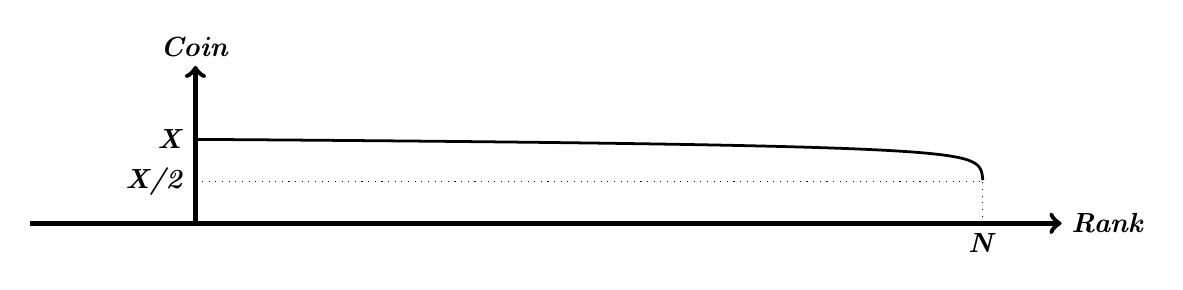
\begin{tikzpicture}
\coordinate (OR) at (0.00, 0.00);
\coordinate (LX) at (-2.10, 0.00); % left x
\coordinate (RX) at (11.00, 0.00); % right x
\coordinate (BY) at (0.00, 0.00); % bottom y
\coordinate (TY) at (0.00, 2.00); % top y
\draw[->][line width=1.75pt] (LX) -- (RX);
\node[right,black] at (11,0) {\textbf{\textit{Rank}}};
\draw[->][line width=1.75pt] (BY) -- (TY);
\node[above,black] at (0, 2) {\textbf{\textit{Coin}}};
\draw[dotted] (0,0.533210267)--(10,0.533210267);
\draw[dotted] (10,0)--(10,0.533210267);
\node[below,black] at (10, 0) {\textbf{\textit{N}}};
\node[left,black] at (0, 0.533210267) {\textbf{\textit{X/2}}};
\node[left,black] at (0, 1.066420536) {\textbf{\textit{X}}};
\draw[black, line width=1.00pt, domain=0:10.00,samples=3000] plot[smooth](\x, {.066598275 * ln(3001-\x * 300) + .533210267});
\end{tikzpicture}
\caption{DIP Reward Distribution Curve}
\label{fig:dipdis}
\end{figure}

DIP rewards will be calculated separately and distributed by each node. Assuming that one block in Nebulas is generated every S second (s),
DIP rewards will be calculated once every 24*7*3600/S blocks for all nodes, and will be distributed to the corresponding smart contract cash-out addresses.

In order to encourage the diversity of Nebulas ecological smart contracts and stimulate outstanding results of more new developers, DIP stipulates that each smart contract can be rewarded up to K time(s). DIP will select Top N smart contracts qualified for rewards according to ranking so as to promote the development of the ecology construction of blockchain applications.

\subsection{Experimental Results}
\label{dip:economic}

We collected the transaction data occurred in May 2017 from Ethereum and calculated the DIP ranking of the first week, as shown in Table \ref{table:dip}.

\begin{table}[h]
\centering
\begin{threeparttable}[b]
\caption{Top 10 of DIP Ranking Results of the First Week in May 2017\tnote{1}}
\label{table:dip}
\begin{tabular}{ccc} \toprule
    {Contract~Address} & {Score} & {Description\tnote{2}} \\ \midrule
0xa74476443119a942de498590fe1f2454d7d4ac0d & 264456363.0 & GolemToken \\
0x49edf201c1e139282643d5e7c6fb0c7219ad1db7 & 207900181.0 & TokenCard-ICO \\
0x48c80f1f4d53d5951e5d5438b54cba84f29f32a5 & 129625776.0 & REP-Augur-OLD \\
0x6810e776880c02933d47db1b9fc05908e5386b96 & 108324489.0 & Gnosis-TokenContract \\
0x6090a6e47849629b7245dfa1ca21d94cd15878ef & 54429341.0 & ENS-Registrar \\
0x607f4c5bb672230e8672085532f7e901544a7375 & 48526808.0 & RLC \\
0x8d12a197cb00d4747a1fe03395095ce2a5cc6819 & 46498412.0 & etherdelta\_2 \\
0xf7b098298f7c69fc14610bf71d5e02c60792894c & 43746158.0 & GUPToken \\
0xaaaf91d9b90df800df4f55c205fd6989c977e73a & 42026627.0 & TokenCardContract \\
0xaec2e87e0a235266d9c5adc9deb4b2e29b54d009 & 41427314.0 & singularDTVToken \\
\bottomrule
\end{tabular}
\begin{tablenotes}
  \small
  \item[1] block range [3629091, 3665815]
  \item[2] from etherscan.io
\end{tablenotes}
\end{threeparttable}
\end{table}

It can be seen that the top-ranked contracts are more famous and more active in the calculation cycle, which are in line with our original intention of motivating the eco-builders.

\subsection{Cheating Analysis}
\label{dip:sybil}

The smart contract can only be called passively. Therefore, if a cheater wants to increase his/her smart contract ranking, he/she has to find sufficient high-NR ranking accounts to call his/her contract.

First of all, it will be impossible for cheaters to improve their DIP ranking at the cost of zero. Provided that a cheater wants to improve his/her ranking of Contract C and forges a great number of accounts for it. However, when SCS is calculated in Equation \ref{formula:dip:scs}, only Top X of SCS of calling in the NR ranking is greater than 0, while the NR ranking of his/her newly forged accounts will be outside Top X. Even if Contract C is called, it will impose no impact on the DIP ranking.

Secondly, if a cheater is willing to pay a certain price for improving his/her DIP ranking of the contract, two options are available for him/her. The first one is to forge accounts with high NR and call Contract C at his/her cost so as to improve the ranking of Contract C. It has been analyzed for forging accounts with the high NR in \refsec{subsec:robust}. To improve the NR for each account, a vast sum of money is required to forge the special topology of such account. Besides, as NR is updated periodically, it will be very expensive to maintain high NR. The second one is to find a great number of accounts with high NR and persuade or bribe their owners to call Contract C. However, it is difficult for such off-chain actions to be scaled up. What's worse, these accounts with high NR found by the cheater at a great cost will account for only a small part of Top X, which will impose almost no impact on really outstanding contracts.